%----------------------------------------------------------------------------
%
% 
% 
%
%----------------------------------------------------------------------------
%----------------------------------------------------------------------------
%----------------------------------------------------------------------------

\ProvidesFile{proposal.tex}
\documentclass[cameraready]{acmsiggraph-awb}
\usepackage[scaled=.92]{helvet}
\usepackage{times}
\usepackage{algorithm}
\usepackage{algorithmic}

\usepackage[pdftex]{graphicx} \pdfcompresslevel=9

\usepackage{parskip}

\usepackage[labelfont=bf,textfont=it]{caption}

\usepackage{amsmath}
\usepackage{amssymb}
\usepackage{wasysym}
\usepackage{bm}
\usepackage{cite}
\usepackage{enumerate}

\usepackage{url}

% For backwards compatibility to old LaTeX type font selection.
% Uncomment if your document adheres to LaTeX2e recommendations.
\let\rm=\rmfamily    \let\sf=\sffamily    \let\tt=\ttfamily
\let\it=\itshape     \let\sl=\slshape     \let\sc=\scshape
\let\bf=\bfseries

% end of prologue
\usepackage[%
 breaklinks,
 letterpaper,
 bookmarks,
 bookmarksnumbered,
 colorlinks,
 linkcolor={black},
 citecolor={black},
 pdfpagemode={None},
]{hyperref}
\setlength\paperwidth{8.5in}  % Override any random settings...
\setlength\paperheight{11in}

\DeclareMathOperator*{\argmin}{\arg\!\min}


\newcommand{\etal}{et al.}
\newcommand{\hidecomment}[1]{}
\newcommand{\Mueller}{M\"{u}ller\ }
\newcommand{\Bez}{B\'{e}zier\ }
\newcommand{\BM}[1]{\B{#1}}
%\newcommand{\B}[1]{\mbox{\boldmath$#1$}}
%\newcommand{\B}[1]{\textbf{\textit{#1}}}
\newcommand{\B}[1]{\mathit{\mathbf{#1}}}
%\newcommand{\B}[1]{\boldsymbol{#1}}
\newcommand{\Per}{\%}
\newcommand{\Unit}[1]{{\mbox{$\,\mathrm{#1}$}}}
\newcommand{\Snit}[1]{{\mbox{\small$\mathrm{#1}$}}}
\newcommand{\Tr}[1]{\mathrm{Tr}\left(#1\right)}
\newcommand{\Hz}{\Unit{Hz}}
\newcommand{\MHz}{\Unit{MHz}}
\newcommand{\GHz}{\Unit{GHz}}
\newcommand{\Sec}{\Unit{sec}}
\newcommand{\SPF}{\Unit{sec/frame}}
\newcommand{\Min}{\Unit{min}}
\newcommand{\Max}{\Unit{max}}
\newcommand{\M}{\Unit{m}}
\newcommand{\Nab}{\B{\nabla}}
\newcommand{\TP}{^\mathsf{T}}

\newcommand{\Dist}{\mbox{dist}}

\newcommand{\figureTopBot}[1]{
  \begin{figure}[!tb]{\sloppy #1}\end{figure}
}

\newcommand{\figureTop}[1]{
  \begin{figure}[!t]{\sloppy #1}\end{figure}
}
 
\newcommand{\figureBot}[1]{
  \begin{figure}[!b]{\sloppy #1}\end{figure}
}

\newcommand{\figureWideTop}[1]{
  \begin{figure*}[!t]{\sloppy #1}\end{figure*}
}

\newcommand{\eqAlgn}{\!\!&\!\!}

\newcommand{\Eref}[1]{Equation~(\ref{#1})}
\newcommand{\Erefs}[2]{Equations~(\ref{#1}) and (\ref{#2})}
\newcommand{\eref}[1]{Equation~(\ref{#1})}
\newcommand{\erefs}[2]{Equations~(\ref{#1}) and (\ref{#2})}
\newcommand{\Sref}[1]{Section~\ref{#1}}
\newcommand{\sref}[1]{Section~\ref{#1}}
\newcommand{\fref}[1]{Figure~\ref{#1}}
\newcommand{\frefAND}[2]{Figures~\ref{#1} and~\ref{#2}}
\newcommand{\frefs}[2]{Figures~\ref{#1} and~\ref{#2}}
\newcommand{\frefss}[3]{Figures~\ref{#1}, \ref{#2}, and~\ref{#3}}
\newcommand{\Fref}[1]{Figure~\ref{#1}}
\newcommand{\Frefs}[2]{Figures~\ref{#1} and~\ref{#2}}
\newcommand{\Frefss}[3]{Figures~\ref{#1}, \ref{#2}, and~\ref{#3}}
\newcommand{\tref}[1]{Table~\ref{#1}}

\renewcommand{\labelenumi}{\arabic{enumi}.}
\renewcommand{\labelenumii}{\alph{enumii}.}
\renewcommand{\labelenumiii}{\roman{enumiii}.}

\newenvironment{algstep}{%
  \begin{enumerate}%
    \setlength{\itemsep}{0in}%
    \setlength{\partopsep}{0in}%
    \setlength{\topsep}{0in}%
}{\end{enumerate}}





\onlineid{papers\_0632}
\newcommand{\theTitle}{GPU Accelerated Point-Based Elastoplastic Solid Simulation}

\title{\theTitle}

\author{
	Ben Jones \and Kyle Hansen}

\newcommand{\theKeywords}{%
  viscoelastic materials, point-based animation, natural phenomena, physics-based animation.%
}


\begin{document}

\teaser{\begin{centering}
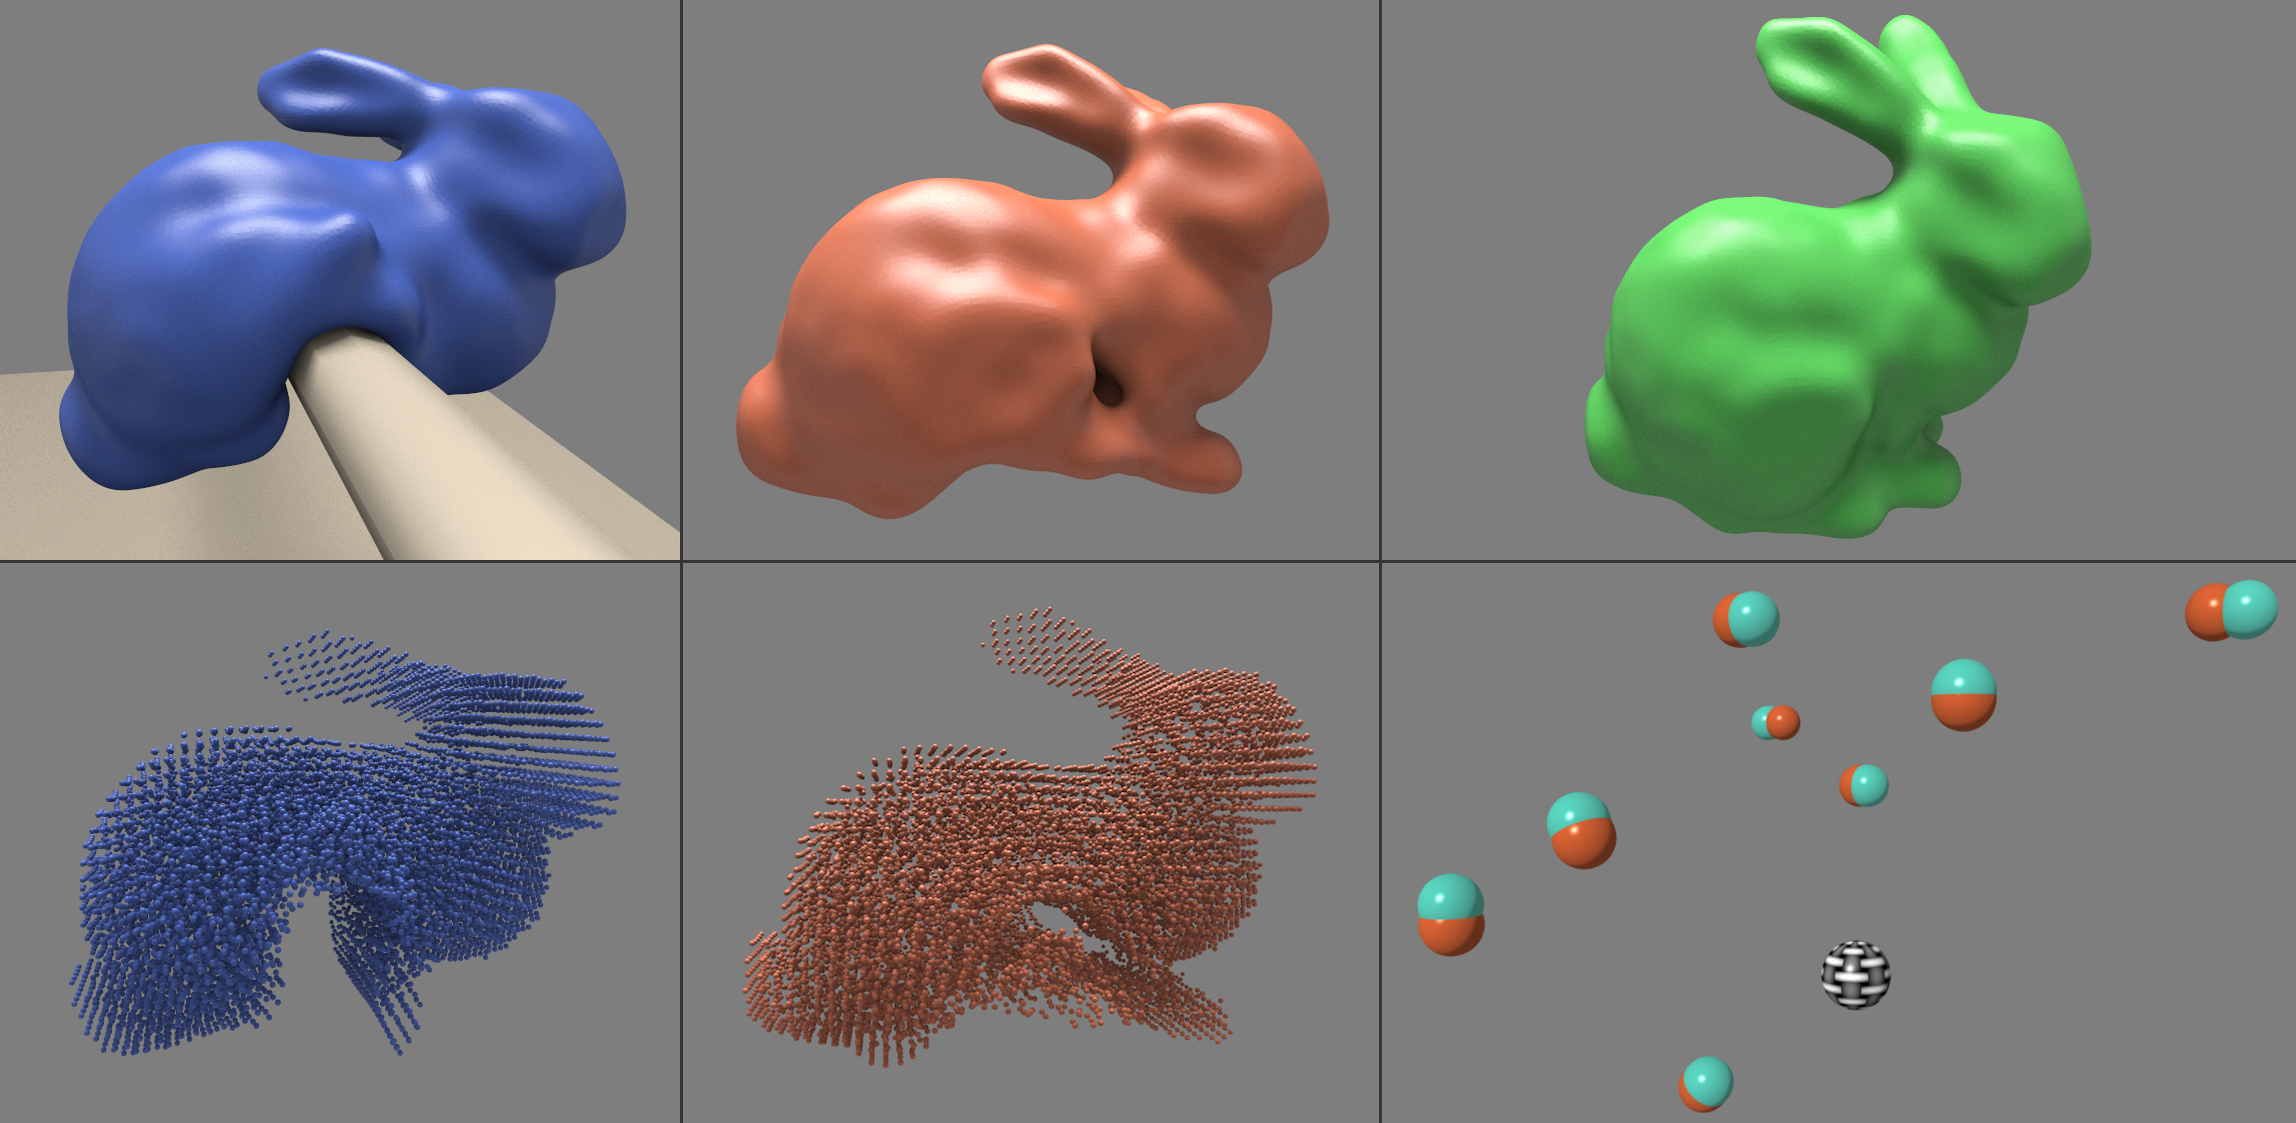
\includegraphics[width=6.1in]{Figures/teaser.png}
\caption{Sample frames from a sequential, point-based elastoplastic simulator, which we hope to accelerate with a GPU implementation.}
\label{fig:teaser}
\end{centering}
}

\maketitle




\section{Team members}

\begin{itemize}

\item Ben Jones: Part of the team that implemented the sequential version of this algorithm, working with Adam Bargteil on graphics simulation research.
Will be focusing on the core algorithm parallelization.

\item Kyle Hansen: Computing Masters Student in the Graphics and Visualization Track.  
2+ years of real world programming experience as an electronics engineer.  
Hobby game programmer.  
Will be primarily concerned with the real time openGL rendering of simulation results.

\end{itemize}

\section{Problem Description}

Simulating deformable solids is important for creating visual effects.  To generate compelling effects, we need to be able to handle materials across the entire spectrum from highly elastic, to totally plastic.  Using finite element methods with volumetric meshes (often tetrahedral) is a common approach, but large plastic deformation creates poorly conditioned tets.  To handle this, complicated volumetric remeshing is necessary to maintain stability and accuracy.  Recently, several point based methods have been proposed to avoid these expensive/complex operations.  However, these methods often support only one end of the spectrum, elastic or plastic materials, but not both  \cite{meuller}, \cite{dan}.  Recently, \cite{us} proposed a new point based technique that handles materials across the range between elastic and plastic.  The goal of our project is to improve performance of their method by performing as much computation as possible on the GPU.  

During the simulation, we maintain the objects world configuration, a set of nearest neighbors for each particle, and least squares fit of the global reference configuration.  At each simulation time step, we perform the following steps:
\newpage
\begin{itemize}

\item compute deformation gradient, per particle
\begin{itemize}
\item factor gradient into elastic and plastic components
\item apply elastic and body (gravity) forces
\item apply plastic deformation to vectors to all neighbors of a particle
\end{itemize}
\item integrate elastic forces
\begin{itemize}
\item perform explicit integration step of elastic and body forces
\item perform implicit damping force solve (conjugate gradient (CG) solve of a sparse matrix)
\end{itemize}
\item compute new world reference configuration (sparse least squares solve using CG)
\item compute per particle local error in global reference configuration 
\item update particle neighborhoods (construct KD tree and do bounded nearest neighbor lookups)
\item resolve obstacle collisions
\item (optional) render current simulation frame (using openGL)
\item write particle positions to file
\end{itemize}


For more details please refer to \cite{us}.

\section{Suitability for GPU implementation}

Since the simulation is particle based, there is no explicit connectivity in the object, and hence, few data dependencies.  
Most steps involve computing 3x3 matrices based on local information, or information from neighbor particles.  
Within these steps, very little synchronization is required, since most writes are to a particle's own data. 
Therefore, most of the algorithm is inherently parallel, and we expect to see large speedups by performing operations on the GPU.  

The two global solves involve solving sparse symmetric positive definite matrices using CG.  Each iteration requires a matrix multiply and a few dot products.  As stated in class, these operations don't perform particularly well on a GPU, but easily outperform CPU implementations.

The KD tree data structure used for the nearest neighbor lookup is not well suited to parallelization.  
Therefore, it may be necessary to perform the nearest neighbors lookup on the CPU, in which case, each time neighbors are updated, we would need to copy the array of reference space positions from GPU to CPU, and copy the array of neighbor information to the GPU.  The sequential implementation performs this copy every 10 timesteps, so it is unlikely that this will be a significant bottleneck.  

For real time rendering, we hope to share buffers between CUDA and OpenGL so that there is no copy overhead to render the points.  

There will be some copy overhead for each simulation frame when the points are copied back to the host to be written to a file, 
but the impact is not expected to be significant.

\section{Intellectual Challenges}

We expect the biggest challenges to come from solving the sparse matrices.
These will be large matrices and care will need to be taken to break them up effectively for parallel computation.
That much is relatively straightforward and similar to previous assignments, but it will be further complicated by the use of sparce matrix methods.

Aside from that, much of the simulation parallelization should simply involve converting loops into threaded CUDA functions, 
although atomic operations or other synchronization methods may be necessary when calculating interactions between neighboring particles.

Additionally, there may be some challenges in implementing the openGL rendering of the simulation.  
Such difficulties will be due more to unfamiliarity with the process and libraries rather than it being theoretically difficult, 
since CUDA already has functions that provide the ability to coordinate with openGL for rendering purposes.

%\begin{CRcatlist}
  %\CRcat{I.3.7}{Computer Graphics}{Three-Dimensional Graphics and Realism}{Animation};
  %\CRcat{I.6.8}{Simulation and Modeling}{Types of Simulation}{Animation}.
%\end{CRcatlist}

%\keywordlist


%----------------------------------------------------------------------------
%----------------------------------------------------------------------------




%\let\ORIGCaption\caption
%\renewcommand{\caption}[1]{\vspace{-0.025in}\ORIGCaption{#1}}

%----------------------------------------------------------------------------
%----------------------------------------------------------------------------


%\bibliographystyle{acmsiggraph-awb}
%\bibliography{monalisa}

\end{document}

